%!TEX program = xelatex
\documentclass[dvipsnames, svgnames,a4paper,11pt]{article}
% ----------------------------------------------------
%   中山大学物理与天文学院本科实验报告模板
%   作者:Huanyu Shi,2019级
%   知乎:https://www.zhihu.com/people/za-ran-zhu-fu-liu-xing
%   Github:https://github.com/Huanyu-Shi/SYSU-SPA-Labreport-Template
%   Last update : 2023.4.10
% ----------------------------------------------------

% ----------------------------------------------------- 
%	加边框的命令
%	参考:https://tex.stackexchange.com/questions/531559/how-to-add-the-page-border-for-first-two-pages-in-latex
\usepackage{tikz}
\usetikzlibrary{calc}
\usepackage{eso-pic}
\AddToShipoutPictureBG{%
\begin{tikzpicture}[overlay,remember picture]
\draw[line width=0.6pt] % 边框粗细
    ($ (current page.north west) + (0.6cm,-0.6cm) $)
    rectangle
    ($ (current page.south east) + (-0.6cm,0.6cm) $); % 边框位置
\end{tikzpicture}}


\usepackage{xcolor}
\definecolor{c1}{HTML}{2752C9} % 目录颜色
\definecolor{c2}{RGB}{190,20,83} % 引用颜色

\usepackage{ctex}
\usepackage[top=28mm,bottom=28mm,left=15mm,right=15mm]{geometry}
\usepackage{hyperref} 
\hypersetup{
	colorlinks,
	linktoc = section, % 超链接位置,选项有section, page, all
	linkcolor = c1, % linkcolor 目录颜色
	citecolor = c1  % citecolor 引用颜色
}
\usepackage{amsmath,enumerate,multirow,float}
\usepackage{tabularx}
\usepackage{tabu}
\usepackage{subfig}
\usepackage{fancyhdr}
\usepackage{graphicx}
\usepackage{wrapfig}  
\usepackage{physics}
\usepackage{appendix}
\usepackage{amsfonts}

%
\usepackage{tcolorbox}
\tcbuselibrary{skins,breakable}
\newtcolorbox{tbox}[2][]{
    colframe=black!70!,
    breakable,
    enhanced,
	boxrule =0.5pt,
    title = {#2},
    fonttitle = \large\kaishu\bfseries,
	drop fuzzy shadow,
    #1
}
\newtcolorbox[auto counter,number within=section]{question}[1][]{
  top=2pt,bottom=2pt,arc=1mm,
  boxrule=0.5pt,
%   frame hidden,
  breakable,
  enhanced, %跨页后不会显示下边框
  coltitle=c1!80!gray,
  colframe=c1,
  colback=c1!3!white,
  drop fuzzy shadow,
  title={思考题~\thetcbcounter:\quad},
  fonttitle=\bfseries,
  attach title to upper,
  #1
}
\newcommand{\setLhead}[1]{%
  \lhead{{\color{gray}\kaishu #1}} % 定义新的命令,设置右边页眉的内容
}
\newcommand{\setRhead}[1]{%
  \rhead{{\color{gray}\kaishu #1}} % 定义新的命令,设置右边页眉的内容
}
% ---------------------------------------------------------------------
%	利用cleveref改变引用格式,\cref是引用命令
\usepackage{cleveref}
\crefformat{figure}{#2{\textcolor{c2}{图 #1}}#3} % 图片的引用格式
\crefformat{equation}{#2{(\textcolor{c2}{#1})}#3} % 公式的引用格式
\crefformat{table}{#2{\textcolor{c2}{表 #1}}#3} % 表格的引用格式


% ---------------------------------------------------------------------
%	页眉页脚设置
\fancypagestyle{plain}{\pagestyle{fancy}}
\pagestyle{fancy}
\setLhead{中山大学物理与天文学院基础物理实验预习报告}
%\lhead{\kaishu 中山大学物理与天文学院物理实验\uppercase\expandafter{\romannumeral3}} % 左边页眉,学院 + 课程
%\rhead{{\color{gray}\kaishu Template 实验报告模板}} % 右边页眉,实验报告标题
\setRhead{实验1\hspace{1pt}冰的熔化热测量}
\cfoot{\thepage} % 页脚,中间添加页码


% ---------------------------------------------------------------------
%	对目录、章节标题的设置
\renewcommand{\contentsname}{\centerline{\huge 目录}}
\usepackage{titlesec}
\usepackage{titletoc}
% \titleformat{章节}[形状]{格式}{标题序号}{序号与标题间距}{标题前命令}[标题后命令]
\titleformat{\section}{\centering\LARGE\songti}{}{1em}{}

% ---------------------------------------------------------------------
%   listing代码环境设置
\usepackage{listings}
\lstloadlanguages{python}
\lstdefinestyle{pythonstyle}{
backgroundcolor=\color{gray!5},
language=python,
frameround=tftt,
frame=shadowbox, 
keepspaces=true,
breaklines,
columns=spaceflexible,                   
basicstyle=\ttfamily\small, % 基本文本设置,字体为teletype,大小为scriptsize
keywordstyle=[1]\color{c1}\bfseries, 
keywordstyle=[2]\color{Red!70!black},   
stringstyle=\color{Purple},       
showstringspaces=false,
commentstyle=\ttfamily\scriptsize\color{green!40!black},%注释文本设置,字体为sf,大小为smaller
tabsize=2,
morekeywords={as},
morekeywords=[2]{np, plt, sp},
numbers=left, % 代码行数
numberstyle=\it\tiny\color{gray}, % 代码行数的数字字体设置
stepnumber=1,
rulesepcolor=\color{gray!30!white}
}




% ---------------------------------------------------------------------
%	其他设置
\def\degree{${}^{\circ}$} % 角度
\graphicspath{{./images/}} % 插入图片的相对路径
\allowdisplaybreaks[4]  %允许公式跨页 % 导入模板的相关设置
\usepackage{lipsum}
\usepackage{indentfirst}
\usepackage{pdfpages}
\usepackage{multirow}
\usepackage{subfig}
\usepackage{graphicx}
\usepackage{float} 
\usepackage{booktabs}
\usepackage{enumerate}
\renewcommand{\d}{\mathrm{d}}
\newcommand{\upcite}[1]{\textsuperscript{\textsuperscript{\cite{#1}}}}


%---------------------------------------------------------------------
%	正文
%---------------------------------------------------------------------
\setRhead{光栅常数及光波波长的测量实验}%实验名称
\begin{document}


\begin{table}
	\renewcommand\arraystretch{1.7}
	\begin{tabularx}{\textwidth}{
		|X|X|X|X
		|X|X|X|X|}
	\hline
	\multicolumn{2}{|c|}{预习报告}&\multicolumn{2}{|c|}{实验记录}&\multicolumn{2}{|c|}{分析讨论}&\multicolumn{2}{|c|}{总成绩}\\
	\hline
	 & &  & &  & &  & \\
	\hline
	\end{tabularx}
\end{table}


\begin{table}
	\renewcommand\arraystretch{1.7}
	\begin{tabularx}{\textwidth}{|X|X|X|X|}
	\hline
	专业:& 物理学类 &年级:& 2023级\\
	\hline
	姓名:& 姚昊廷  & 学号:&22322091\\
	\hline
	实验时间:& 2024.11.28& 教师签名:& \\
	\hline
	\end{tabularx}
\end{table}

\begin{center}
	\LARGE 光栅常数及光波波长的测量实验
\end{center}

\textbf{【实验报告注意事项】}
\begin{enumerate}
	\item 实验报告由三部分组成:
	\begin{enumerate}
		\item 预习报告:(提前一周)认真研读\underline{\textbf{实验讲义}},弄清实验原理;实验所需的仪器设备、用具及其使用(强烈建议到实验室预习),完成课前预习思考题;了解实验需要测量的物理量,并根据要求提前准备实验记录表格(第一循环实验已由教师提供模板,可以打印)。预习成绩低于10分(共20分)者不能做实验。
	    \item 实验记录:认真、客观记录实验条件、实验过程中的现象以及数据。实验记录请用珠笔或者钢笔书写并签名(\textcolor{red}{\textbf{用铅笔记录的被认为无效}})。\textcolor{red}{\textbf{保持原始记录,包括写错删除部分,如因误记需要修改记录,必须按规范修改。}}(不得输入电脑打印,但可扫描手记后打印扫描件);离开前请实验教师检查记录并签名。
	    \item 分析讨论:处理实验原始数据(学习仪器使用类型的实验除外),对数据的可靠性和合理性进行分析;按规范呈现数据和结果(图、表),包括数据、图表按顺序编号及其引用;分析物理现象(含回答实验思考题,写出问题思考过程,必要时按规范引用数据);最后得出结论。
	\end{enumerate}
	\textbf{实验报告就是将预习报告、实验记录、和数据处理与分析合起来,加上本页封面。}
	\item 每次完成实验后的一周内交\textbf{实验报告}(特殊情况不能超过两周)。
	\item 除实验记录外,实验报告其他部分建议双面打印。
\end{enumerate}

\textbf{【注意事项】}\\
一、验证多普勒效应实验设备安装时注意事项:
\begin{enumerate}
    \item 实验中{\color{red}禁止用手触摸或擦拭光栅和平面镜等光学元件};
    \item 汞灯不用时请关闭,以{\color{red}防止汞灯的紫外长时间直射到眼睛}!
    \item \textbf{\color{red}请根据讲义内容提前阅读《基础物理实验(沈韩主编)》中的相关章节}。
\end{enumerate}

\clearpage
\tableofcontents
\clearpage

\setcounter{section}{0}
\section{光栅常数及光波波长的测量实验\ \textbf{预习报告}}
	
\subsection{实验目的}
\begin{enumerate}
    \item 了解分光计的构造,原理及其调节方法。
	\item 了解光栅的构造,观测光栅的衍射现象并了解其基本原理。
	\item 掌握测量光栅常数,光波波长和光栅角色散率的方法。
\end{enumerate}
\subsection{仪器用具}
\begin{table}[htbp]
	\centering
	\renewcommand\arraystretch{1.6}
	% \setlength{\tabcolsep}{10mm}
	\begin{tabular}{p{0.05\textwidth}|p{0.20\textwidth}|p{0.05\textwidth}|p{0.5\textwidth}}
	\hline
	编号& 仪器用具名称 & 数量 &  主要参数(型号,测量范围,测量精度等) \\
	\hline
	1&分光计&1 &KF-JJY\\
	\hline
	2&平面镜 &1&$\phi$36×4\\
	\hline
	3&平面透射光栅&1&1/300mm\\
	\hline
	4&汞灯&1&GP20 Hg\\
	\hline
	5&钠灯&1&GP20 Na\\
	\hline
\end{tabular}
\end{table}

\noindent\textbf{【原理概述】}\\
实验采用平面透射光栅,由宽度为$b$的透光部分与宽度为$d$的等间距的平行缝组成。当单色平行光照到光栅上时,透过狭缝的光线将向各个方向衍射。每条光线与其
相邻的光线光程差为$d\sin\theta$。如果该距离等于波长的整数倍,则光线都同相到达,并获得相长干涉(最大值)。因此,获得衍射光栅的相长干涉的必要条件是:
\begin{equation}
    d\sin\theta=k\lambda,(k=0,\pm1,\pm2\cdots)
    \label{1}
\end{equation}
通常光栅狭缝间距要比双缝干涉的缝间距要小,所以在同样的观测角度范围内,光栅所产生的明条纹更少。

\ref{1}式称为光栅方程,它对垂直照射条件下的透射式和反射式光栅都适用。根据式\ref{1}可知,利用分光计测出各种谱线的衍射角,若已知波长,可得光栅常数;反之,若已知光栅常数,则可以求得波长。\par
\subsection{实验前思考题}
\begin{question}
	简述低压汞灯的发光机理,给出特征谱线,并标明可见光波段谱线所对应的颜色。
	\tcblower
	通过电极放电将汞蒸气电离出离子和电子。离子和电子在电场力作用下各自向两个电极运动,
    运动中与更多的原子碰撞,产生出更多的电子和离子。这个过程中,一些原子会被激发到激发态。
    激发态是一个不稳定的状态,在从激发态跃迁回到低能级时,原子便辐射出光子。
    在电源激励下,激发和跃迁反复进行,就是低压汞灯的发光原理。

    特征谱线主要有\begin{enumerate}
        \item 253.65nm
        \item 296.73nm
        \item 302.15nm
        \item 313.16nm
        \item 334.15nm
        \item 365.01nm
        \item 404.66nm
        \item 407.78nm
        \item 435.84nm,紫色
        \item 546.07nm,绿色
        \item 576.96nm,黄色
        \item 579.06nm,黄色
    \end{enumerate}
\end{question}

\begin{question}
	现有每厘米10,000条线平面透射光栅一个,对于575nm光源,计算其+1、+2级衍射线的角度差。
	\tcblower
	$$d=\frac{l}{N}=10^{-6}m,\lambda=5.75\times10^{-7}m$$
    对于+1级谱线
    $$\sin\theta_1=\frac{\lambda}{d}$$
    对于+2级谱线
    $$\sin\theta_2=\frac{2\lambda}{d}=1.15>1$$
    故不存在+2级谱线。
\end{question}


\clearpage
\setLhead{中山大学物理与天文学院基础物理实验记录}
\begin{table}
	\renewcommand\arraystretch{1.7}
	\centering
	\begin{tabularx}{\textwidth}{|X|X|X|X|}
	\hline
	专业:& 物理学类 &年级:& 2023级 \\
	\hline
	姓名: &姚昊廷& 学号:&22322091  \\
	\hline
	室温:&$22^\circ$C&实验地点:&A508  14\\
	\hline
	学生签名:& & 评分: &\\
	\hline
	实验时间:& 2024.11.28& 教师签名:&\\
	\hline
	\end{tabularx}
\end{table}
\section{光栅常数及光波波长的测量实验\ \textbf{实验记录}}
\subsection{实验内容、步骤、结果}
\subsubsection{实验内容及步骤}
调节分光计:\begin{enumerate}
	\item 望远镜调焦无穷远\begin{enumerate}
		\item 粗调:调节望远镜光轴高低调节螺钉和和载物台调平螺钉,通过目测判断使望远
		镜光轴及载物台基本水平。
		\item 望远镜目镜调焦:接通望远镜照明电源,在目镜中观
		察到分划板下方有一绿色的亮区先逆时针旋转望远镜目镜调焦手轮使分划板刻线完全
		模糊,再顺时针慢慢旋转该子轮,至刻线清晰且无视差.此后
		不要再转动调焦手轮。
		\item 在载物台上放置平面反射镜,使反
		射面与调平螺钉的连线垂直。
		\item 松开游标盘锁紧螺钉 ,稍微转动游标盘,载物台
		上的反射镜随之转动.从目镜观察,可看到一绿色亮斑,若看
		不到反射回来的绿色亮斑,需重新进行粗调。
		\item 看到反射的亮斑后,松开望远镜目镜锁紧螺钉 ,再调节望远镜物镜调焦螺钉,
		前后伸缩目镜筒,使反射亮斑聚焦成一清晰的绿色十字像,并保证反射的亮十字像和分划板
		上黑色十字线无视差,即左右移动头部(视线需保持在望远镜目镜范围内)时,绿色十
		字像和黑色十字的垂直线间的距离d 保持不变.之后调紧目镜锁紧螺钉.无视差调节非常重
		要,确保测量时不因头部位置不同而导致测量结果发生变化.
	\end{enumerate}
	\item 调节望远镜光轴垂直于公共转轴\begin{enumerate}
		\item 粗调:转动游标盘,交替使反射镜的两面正对望远镜,并通过调节望远镜光轴高
		低调节螺钉和载物台调平螺钉,使得反射镜AB 面正对
		望远镜时都能在视场中看到绿色的十字像。
		\item 细调:采用"渐近法"进行细调,选定一个反射面正对望远镜,在目镜视场中观察,绿色十字像的水平
		线通常不与分划板上方的黑色水平线重合,它们之间有一垂直
		距离L 调节望远镜光轴高低调节螺钉,使l 减少一半.然后
		再调节靠近望远镜的载物台调平螺钉,使它们完全重合.
		将游标盘转$180^\circ$ ,观察反射镜反射的绿色十字像,
		若绿色十字像的水平线与分划板上方的黑色水平线不重
		合,它们之间有垂直距离l,则调节望远镜光轴高低调节螺
		钉 ,使距离减少一半:然后再调节靠近望远镜的载物台调平螺钉(此时不能调节上一面调节的调平螺钉),使它们完全重合。如此交替进行多次,使从反射镜任何一反射面反射回来的绿色十字像的水平线均与分划
		板上方的黑色水平线重合,则望远镜的光轴与公共转轴垂直.之后整个望远镜的调节机构不
		能再作调节。
	\end{enumerate}
	\item 调节载物台水平:将平面镜旋转九十度,重复上一步操作,使绿色十字像水平线与分划板上方的黑色水平
		线重合,则载物台水平。
	\item 平行光管调焦无穷远:点亮光源正照狭缝,松开望远镜支架锁紧螺钉,转动望远镜正对平行光管。松开狭缝装置锁紧螺钉,转动狭缝使狭缝垂直. 再前后伸缩狭缝装置,使狭缝在望远镜中成像清晰, 且
	与分划板上的黑色十宇线没有视差,则平行光管对焦无穷远,锁紧狭缝装置的锁紧螺钉。
	\item 调节平行光管光轴垂直于公共转轴:先将狭缝垂直放置,在水平面移动望远镜并从目镜中观察,使狭缝像与分划板的坚直线
	重合。将狭缝转$90^\circ$ ,调平行光管高低调节螺钉 ,使狭缝像与分划板中心的水平线重合,
	则平行光管光轴与公共转轴垂直。
\end{enumerate}
至此,分光计调节完成。

随后在载物台上放置光栅,在固定平行光管和望远镜的前提下,转动游标盘,使光栅表面
反射的绿色十字像的垂直线与望远镜分划板的竖直线重舍,则光栅面与
平行光管轴线垂直.锁紧游标盘制动螺钉,并在后续的实验中保持游标
盘不转动。转动望远镜并在视场中找到光栅的衍射光谱线,调节狭缝的宽
度使谱线明亮、清晰。若发现左右两组光谱的高度不对称,可轻微调节
载物台调平螺钉,直到左右两组谱线的高度一致。

测定光栅常量:\begin{enumerate}
	\item 记录主极亮的位置,即望远镜分划板竖直线与零级谱线(即平行光管狭缝像)重合时
	的位置,需同时记录游标盘上两个游标的读数。
	\item 把望远镜向零级谱线的一边转动,使分划板垂直线与一级光谱中的铀黄线
	($\lambda=589.3$nm) 重合,记录谱线位置若光谱分辨率高时可能观察到两条黄线,这时应取双黄
	线的平均位置。
	\item 继续沿原方向转动望远镜,用相同方法测量二级光谱中铀黄线的位置。
	\item 把望远镜往零级光谱的另一边转动,作与(2) 和(3) 相同的测量。
	\item 把光栅法线左右两边所测同级光谱中的两个衍射角$\phi$求平均后代入式\ref{1} ,求光栅
	常量d. 要求两个$\phi$值之差不超过10',否则需重新调节入射光与光栅面垂直最后求一、二
	级谱线对应的d 值及其不确定度。
\end{enumerate}

测量汞灯波长:将光源更换为汞灯后重复上述操作并记录下各谱线衍射角。
\subsubsection{实验结果}
\begin{table}[H]
	\centering
	\caption{光栅常数测量}
	\label{2}
	\begin{tabular}{ccccc}
		\toprule
		谱线级数&右读数&左读数&衍射角&平均值\\
		\midrule
		0&$327^\circ12'$&$147^\circ12'$&0&0\\
		\midrule
		$+1$&$337^\circ23'$&$157^\circ22'$&$10^\circ10'30''$&\multirow{2}{*}{$10^\circ10'30''$}\\
		 
		$-1$&$317^\circ1'$&$137^\circ2'$&$10^\circ10'30''$&\\
		\midrule
		$+2$&$347^\circ35'$&$167^\circ54'$&$20^\circ42'30''$&\multirow{2}{*}{$20^\circ41'45''$}\\
		 
		$-2$&$306^\circ31'$&$126^\circ31'$&$20^\circ41'$&\\
		\toprule
	\end{tabular}
\end{table}
\begin{table}[H]
	\centering
	\caption{未知光波长测量(绿)}
	\label{3}
	\begin{tabular}{ccccc}
		\toprule
		谱线级数&右读数&左读数&衍射角&平均值\\
		\midrule
		0&$327^\circ10'$&$147^\circ10'$&0&0\\
		\midrule
		$+1$&$336^\circ37'$&$156^\circ37'$&$9^\circ27'$&\multirow{2}{*}{$9^\circ26'$}\\
		 
		$-1$&$317^\circ45'$&$137^\circ45'$&$9^\circ25'$&\\
		\midrule
		$+2$&$346^\circ18'$&$166^\circ18'$&$19^\circ8'$&\multirow{2}{*}{$19^\circ7'$}\\
		 
		$-2$&$308^\circ4'$&$128^\circ4'$&$19^\circ6'$&\\
		\toprule
	\end{tabular}
\end{table}
\begin{table}[H]
	\centering
	\caption{未知光波长测量(紫)}
	\label{4}
	\begin{tabular}{ccccc}
		\toprule
		谱线级数&右读数&左读数&衍射角&平均值\\
		\midrule
		0&$327^\circ10'$&$147^\circ10'$&0&0\\
		\midrule
		$+1$&$334^\circ41'$&$154^\circ40'$&$7^\circ3'30''$&\multirow{2}{*}{$7^\circ3'15''$}\\
		 
		$-1$&$319^\circ40'$&$139^\circ40'$&$7^\circ30'$&\\
		\midrule
		$+2$&$342^\circ25'$&$162^\circ26'$&$15^\circ15'30''$&\multirow{2}{*}{$15^\circ11'45''$}\\
		 
		$-2$&$312^\circ2'$&$132^\circ2'$&$15^\circ8'$&\\
		\toprule
	\end{tabular}
\end{table}
\begin{table}[H]
	\centering
	\caption{未知光波长测量(黄)}
	\label{5}
	\begin{tabular}{ccccc}
		\toprule
		谱线级数&右读数&左读数&衍射角&平均值\\
		\midrule
		0&$327^\circ10'$&$147^\circ10'$&0&0\\
		\midrule
		$+1$&$337^\circ10'$&$157^\circ9'$&$9^\circ59'30''$&\multirow{2}{*}{$9^\circ57'15''$}\\
		 
		$-1$&$317^\circ15'$&$137^\circ15'$&$9^\circ55'$&\\
		\midrule
		$+2$&$347^\circ30'$&$167^\circ30'$&$20^\circ20'$&\multirow{2}{*}{$20^\circ19'$}\\
		 
		$-2$&$306^\circ52'$&$126^\circ52'$&$20^\circ18'$&\\
		\toprule
	\end{tabular}
\end{table}
\subsection{实验过程中遇到的问题记录}
粗调时难以一次调节成功,视野中无绿色十字线。


\clearpage
\setLhead{中山大学物理与天文学院基础物理实验分析与讨论}
\begin{table}
	\renewcommand\arraystretch{1.7}
	\begin{tabularx}{\textwidth}{|X|X|X|X|}
	\hline
	专业:& 物理学 &年级:& 2023级\\
	\hline
	姓名: &姚昊廷& 学号:&22322091 \\
	\hline
    日期:&2024.11.28 & 评分: &\\
	\hline
	\end{tabularx}
\end{table}

\section{光栅常数及光波波长的测量实验\ \textbf{分析与讨论}}
\subsection{光栅常数计算}
 将表\ref{2}中数据代入式\ref{1}中得到
 \begin{align*}
	d_1&=\frac{\lambda}{\sin\theta_1}=3335.88\text{nm}\\
	d_2&=\frac{2\lambda}{\sin\theta_1}=3334.97\text{nm}
 \end{align*}
 则测量均值为
 \begin{align*}
	\overline{d}=\frac{d_1+d_2}{2}=3335.42\text{nm}
 \end{align*}
 实验标准差为
 \begin{align*}
	\delta=0.64\text{nm}
 \end{align*}
\subsection{未知光波波长及角色散率D计算}
\noindent 绿光波长:

将表\ref{3}中数据代入式\ref{1}中得到
 \begin{align*}
	\lambda_1&=\overline{d}\sin\theta_1=546.66\text{nm}\\
	\lambda_2&=\frac{\overline{d}\sin\theta_1}{2}=546.17\text{nm}
 \end{align*}
 平均值为
 \begin{align*}
	\lambda_g=\frac{\lambda_1+\lambda_2}{2}=546.41\text{nm}
 \end{align*}
 实验标准差为
 \begin{align*}
	\delta=0.34\text{nm}
 \end{align*}
 相对误差为
 \begin{align*}
	\frac{546.41-546.07}{546.07}=0.06\%
 \end{align*}

 \noindent 紫光波长:

将表\ref{4}中数据代入式\ref{1}中得到
 \begin{align*}
	\lambda_1&=\overline{d}\sin\theta_1=435.60\text{nm}\\
	\lambda_2&=\frac{\overline{d}\sin\theta_1}{2}=437.14\text{nm}
 \end{align*}
 平均值为
 \begin{align*}
	\lambda_p=\frac{\lambda_1+\lambda_2}{2}=436.37\text{nm}
 \end{align*}
 实验标准差为
 \begin{align*}
	\delta=1.09\text{nm}
 \end{align*}
 相对误差为
 \begin{align*}
	\frac{\lambda_p-435.84}{435.84}=0.1\%
 \end{align*}

 \noindent 黄光波长:

将表\ref{5}中数据代入式\ref{1}中得到
 \begin{align*}
	\lambda_1&=\overline{d}\sin\theta_1=576.56\text{nm}\\
	\lambda_2&=\frac{\overline{d}\sin\theta_1}{2}=579.04\text{nm}
 \end{align*}
 平均值为
 \begin{align*}
	\lambda_y=\frac{\lambda_1+\lambda_2}{2}=577.80\text{nm}
 \end{align*}
 实验标准差为
 \begin{align*}
	\delta=1.75\text{nm}
 \end{align*}
 相对误差为
 \begin{align*}
	\frac{\lambda_y-576.96}{576.96}=0.1\%
 \end{align*}

 \noindent 角色散率:
因为紫光一级衍射角最小,故选取紫光一级衍射计算角色散率
 \begin{align*}
	D_1=\frac{1}{\overline{d}\cos\varphi_1}=3.02\times10^{-4}\text{rad/m}
 \end{align*}

 测得光波长均偏大,误差来源可能有\begin{enumerate}
	\item 测定光栅常量实验中,两条黄线相距太近,未将分划板对准两条谱线均值处,使得测得的光栅常量较大。
	\item 读数时产生的误差。
	\item 计算时数据取舍造成的舍入误差。
	\item 分光计调节存在一定问题,导致存在一定的视差。
 \end{enumerate}
\subsection{实验后思考题}
\begin{question}
	检索文献,列举三种测量光波波长的方法,给出参考文献列表。
	\tcblower
	\begin{enumerate}
		\item 双棱镜干涉法:双棱镜干涉实验利用双棱镜平分波前产生两束相干光,在光屏上形成干涉条纹,利用透镜成像
		法测量虚光源放大像的间距以及对应的物距和像距可准确测量虚光源的间距。通过测量距离虚
		光源较远处且尽量多的干涉条纹的距离再平均可以准确测量干涉条纹的间距。 采用该测量方法可以
		准确得到光的波长。\upcite{ref1}
		\item 少量透明液体放入器皿中,使器皿旋转,透明液体形成凹薄液膜。当待测光入射至凹薄液膜,该薄膜上下表面的反射光相干时,即可发生干涉现象。通过显微镜观察得到干涉图样,依据干涉原理设计出光波长测量装置;以法兰盘做连接件构成机械转台,实现稳定机械旋转,从而达到准确测量目的。\upcite{ref2}
		\item 通过改变在光的传播路径上垂直放置的透明玻璃与光传播方向的角度,使相干光的光程差发生变化;利用干涉条纹与转过角度、透明玻璃厚度之间的关系,通过激光干涉实验能准确测量出光波的波长。\upcite{ref3}
	\end{enumerate}
\end{question}
\clearpage
% ---------------------------------------------------------------------
%   参考文献
%   注:使用参考文献时应按照xelatex->bibtex->xelatex->xelatex顺序进行编译
\phantomsection
\addcontentsline{toc}{section}{参考文献}
\bibliographystyle{unsrt}
\bibliography{myref}
\begin{thebibliography}{9}
	\bibitem{ref1} 沈雨欣,翁存程,蒋丽钦.双棱镜干涉法准确测量钠光波长[J].大学物理实验,2023,36(03):40-43.DOI:10.14139/j.cnki.cn22-1228.2023.03.008.
	\bibitem{ref2} 牟泉润,孙丽媛,杜月棋,等.基于干涉原理的光波长测量装置设计[J].大学物理实验,2021,34(06):80-83+89.DOI:10.14139/j.cnki.cn22-1228.2021.06.018.
	\bibitem{ref3} 王仁洲,杨涛.一种用激光干涉测量光波波长的新方法[J].大学物理实验,2014,27(06):41-43.DOI:10.14139/j.cnki.cn22-1228.2014.06.014.
\end{thebibliography}


%\clearpage
\appendix
\appendixpage
\addappheadtotoc
%\subsection*{相图代码}
%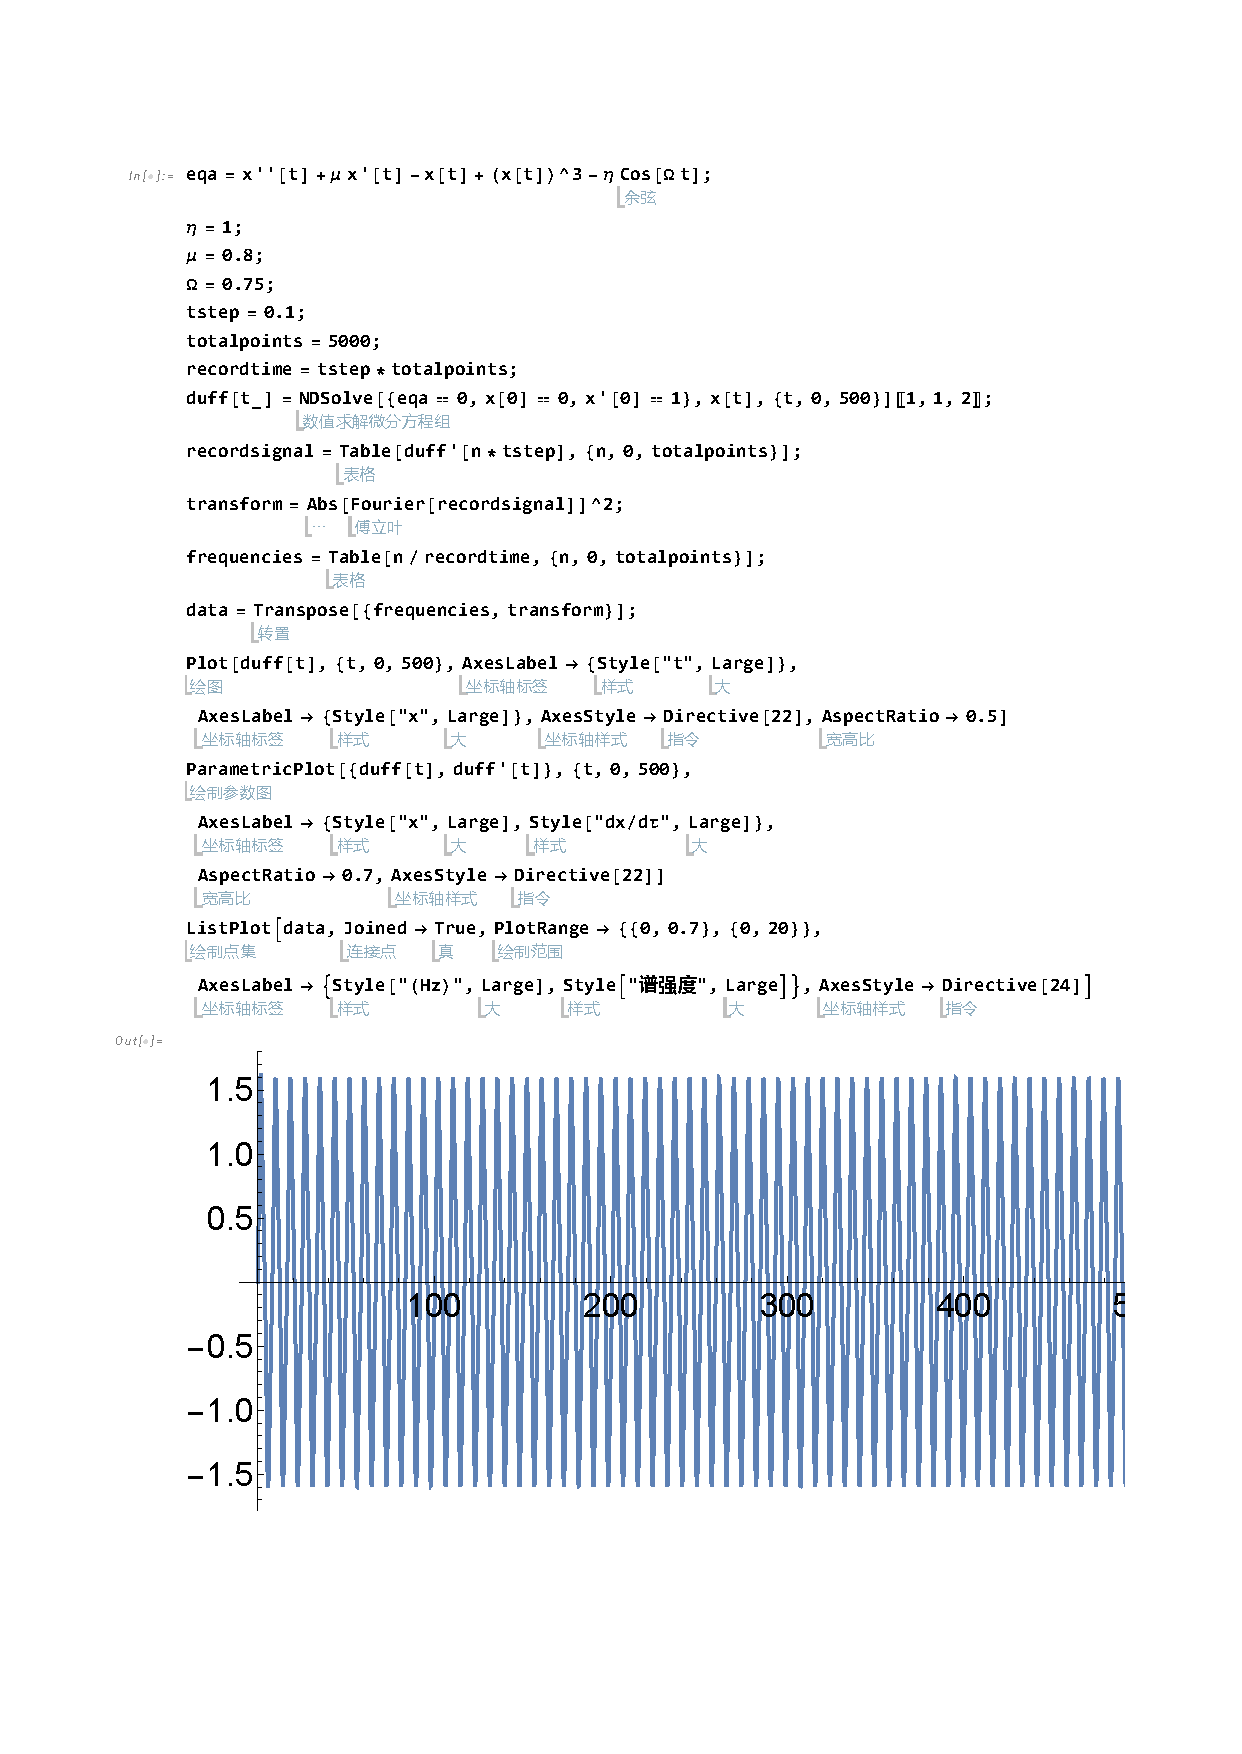
\includepdf[pages=-]{chaos.pdf}
\subsection*{原件}
%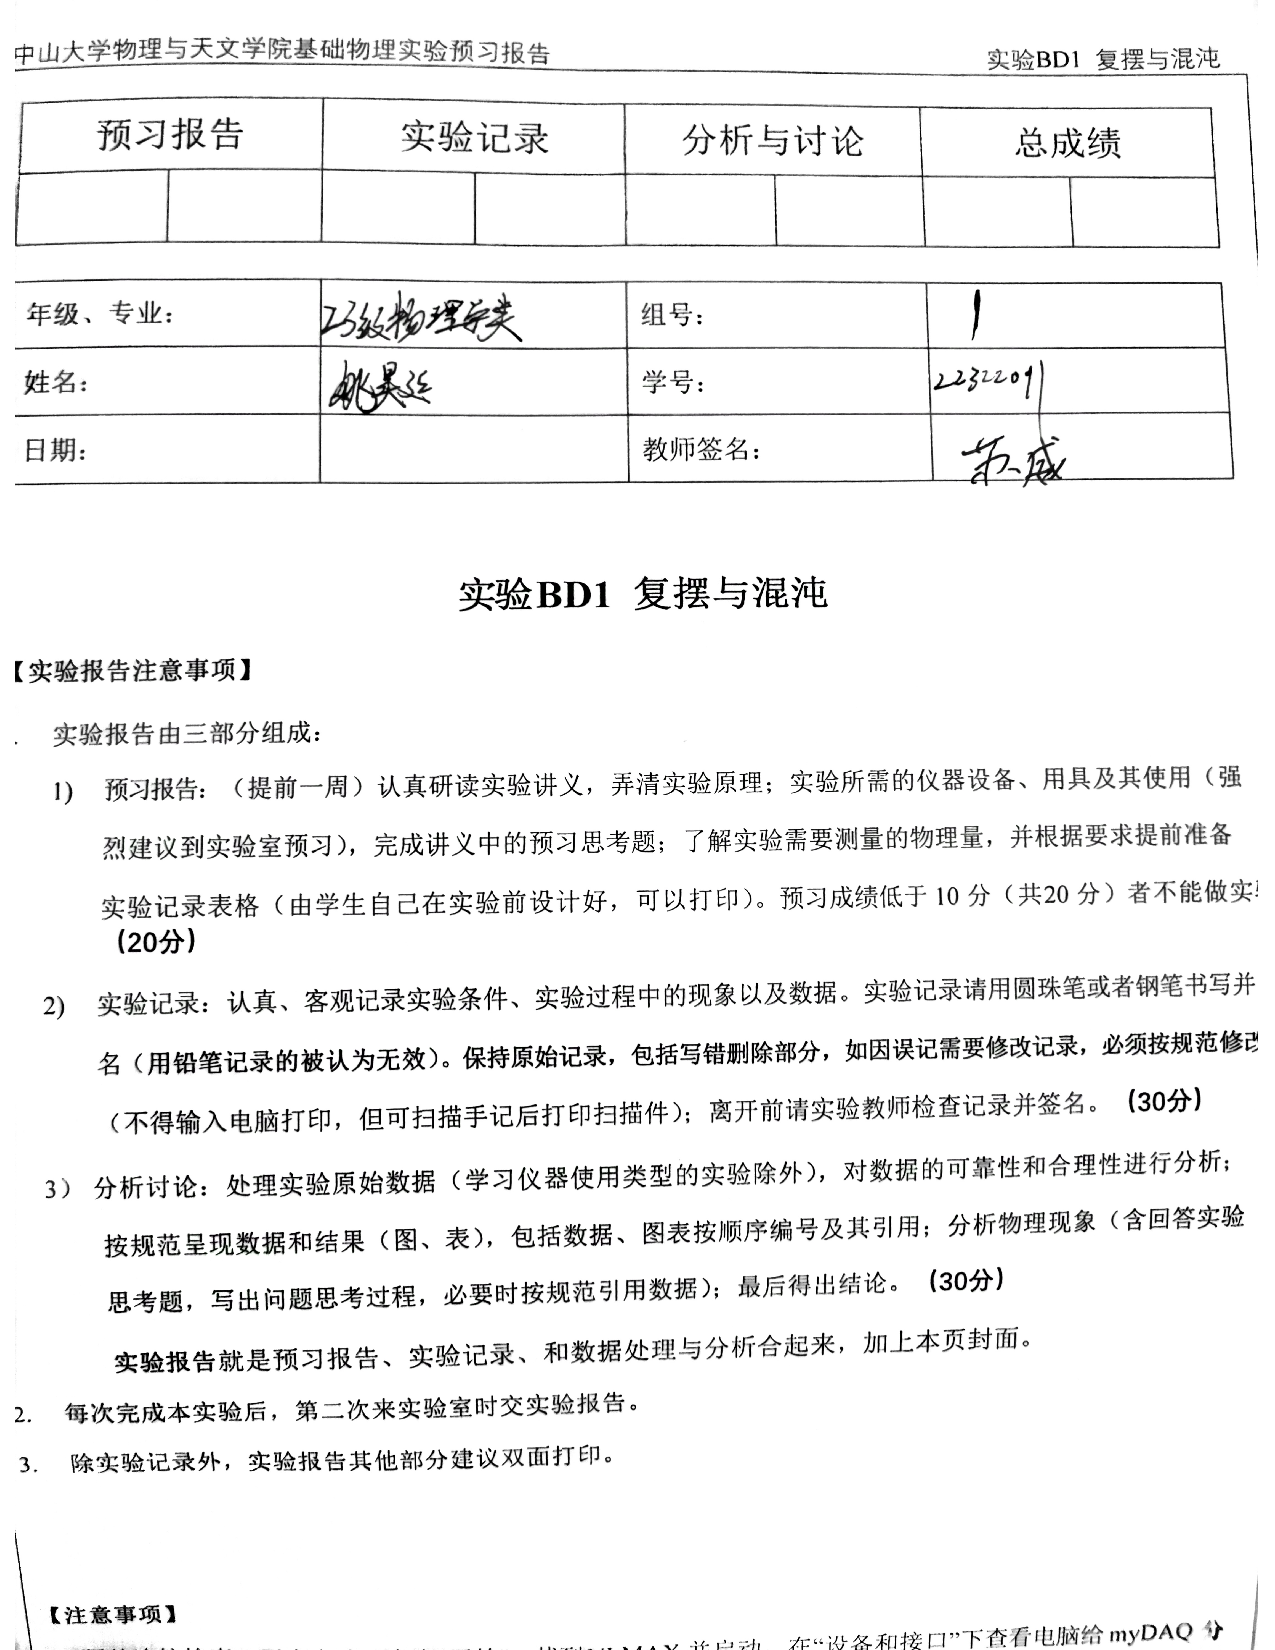
\includepdf[pages=-]{实验3原件.pdf}
\begin{figure}[H]
	\centering
	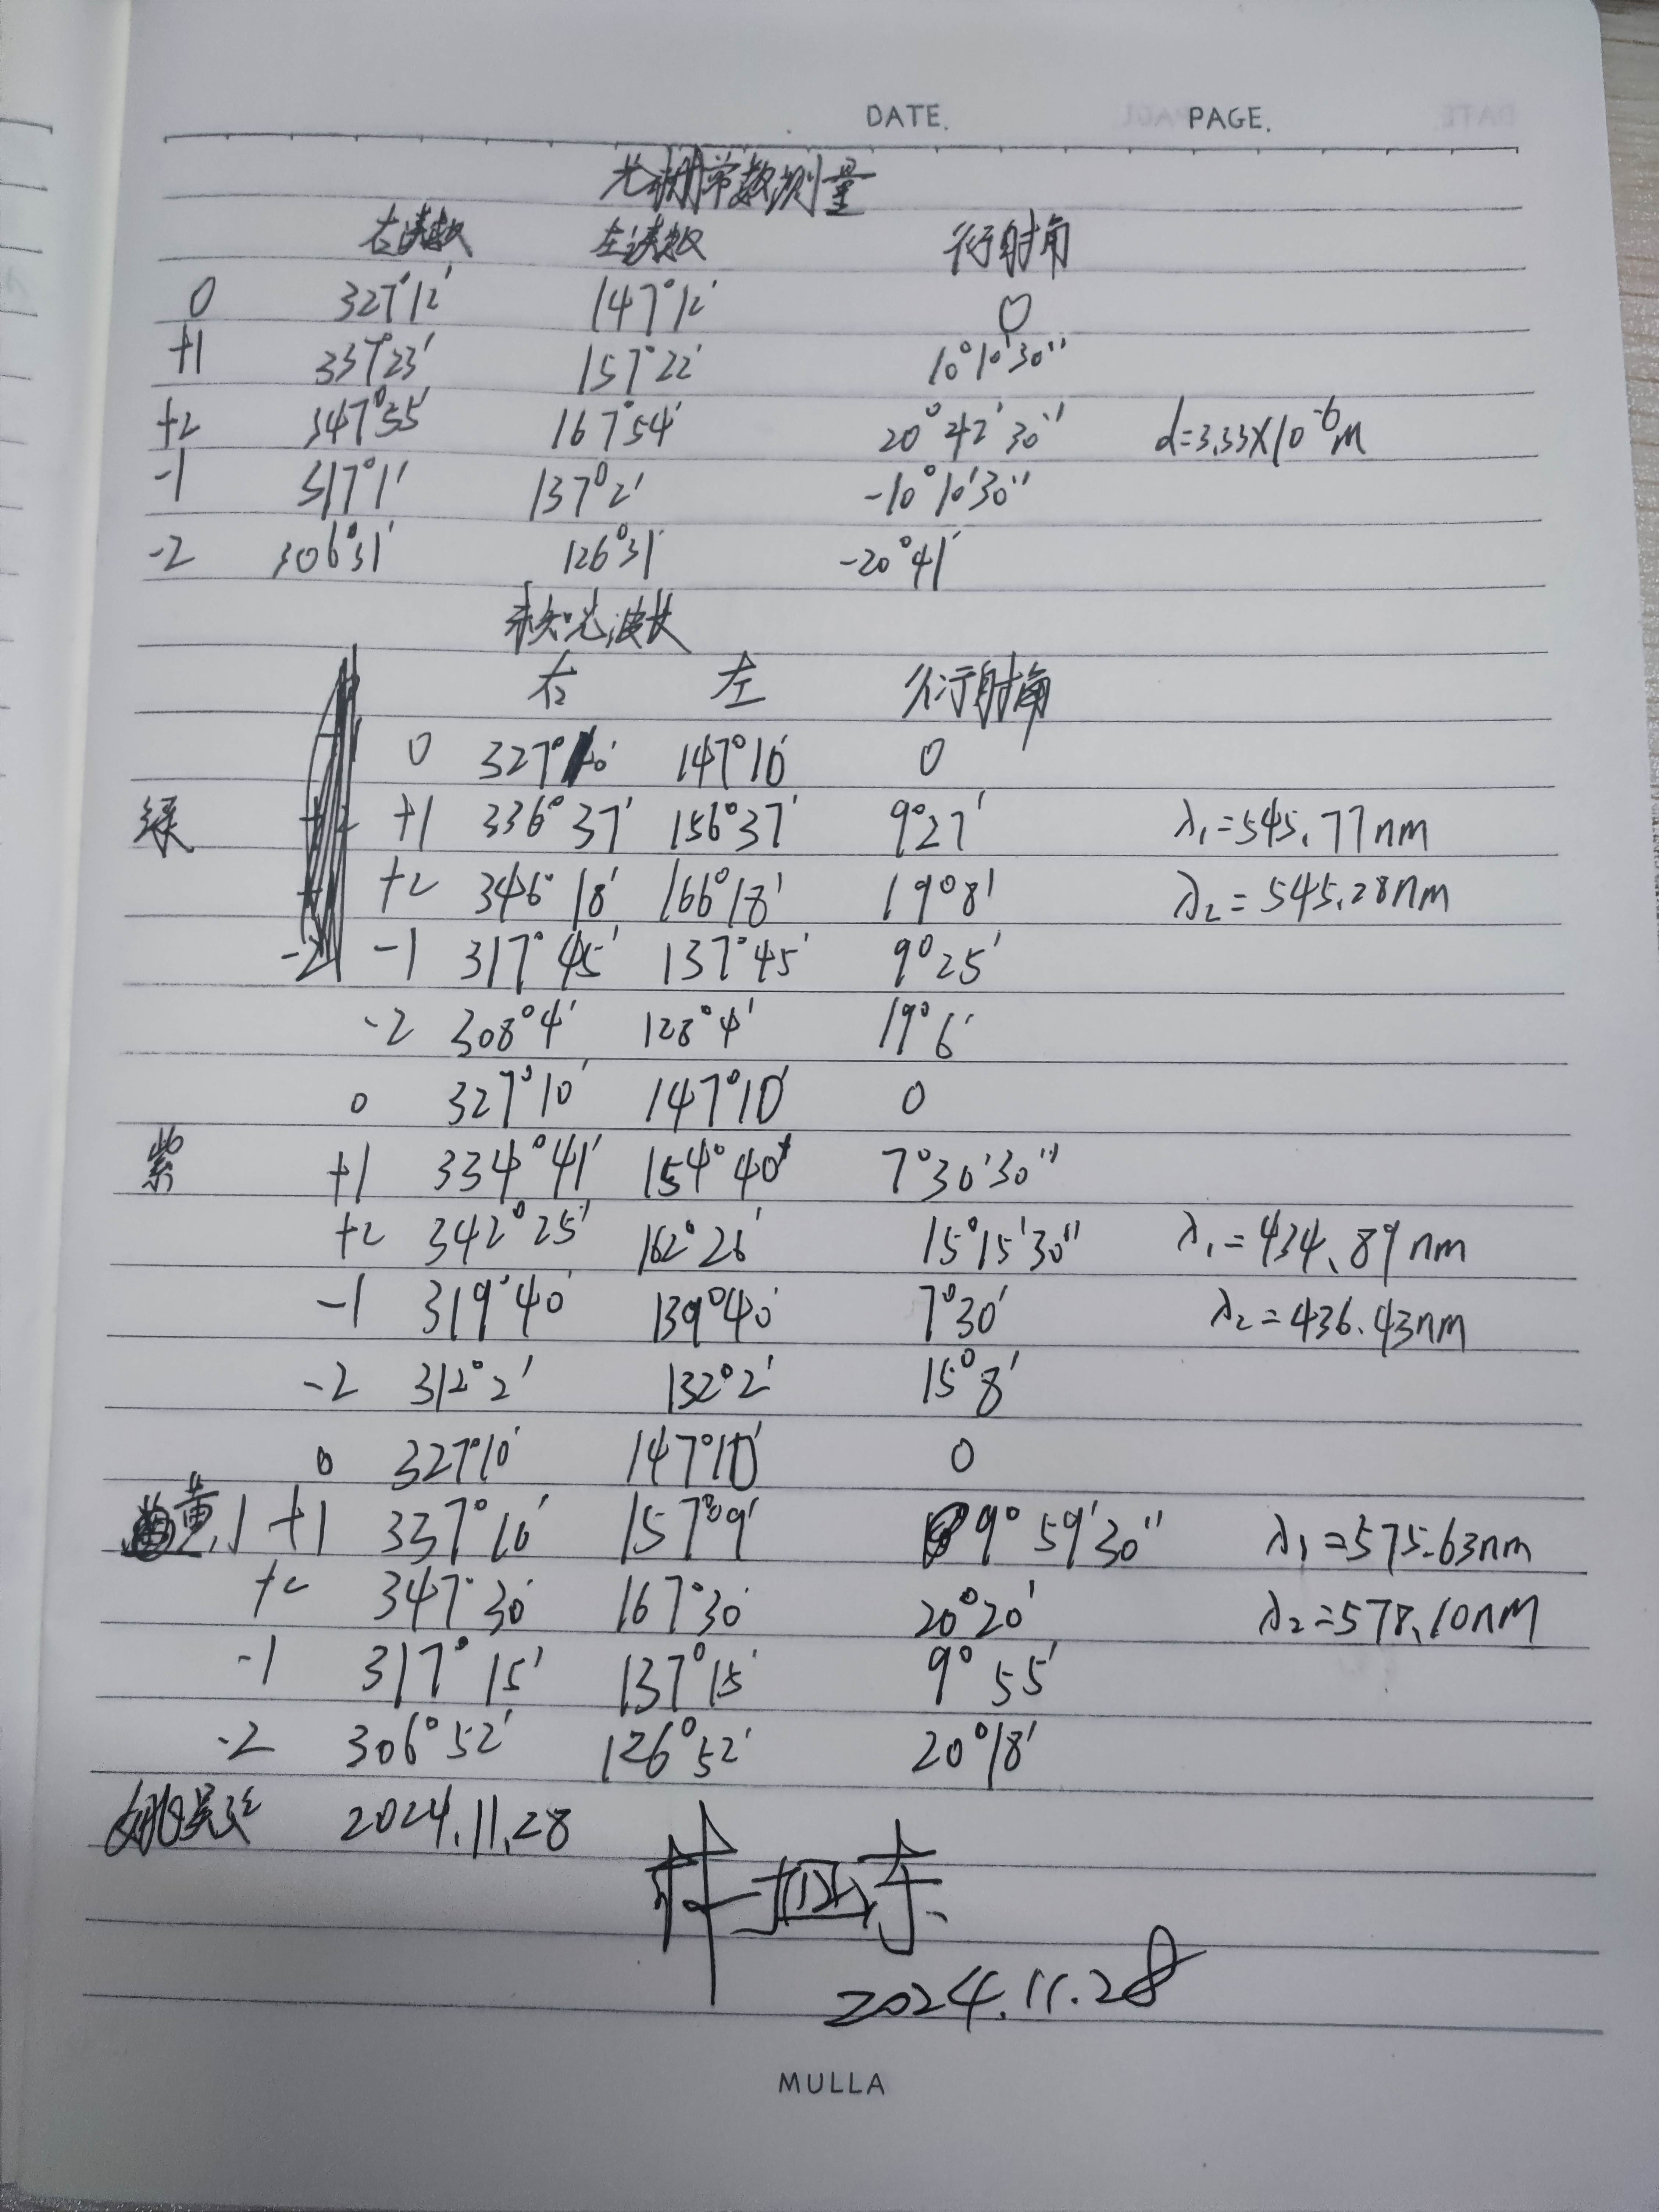
\includegraphics[width=\textwidth]{光栅数据.jpg}
\end{figure}

%\begin{figure}[H]
%	\centering
%	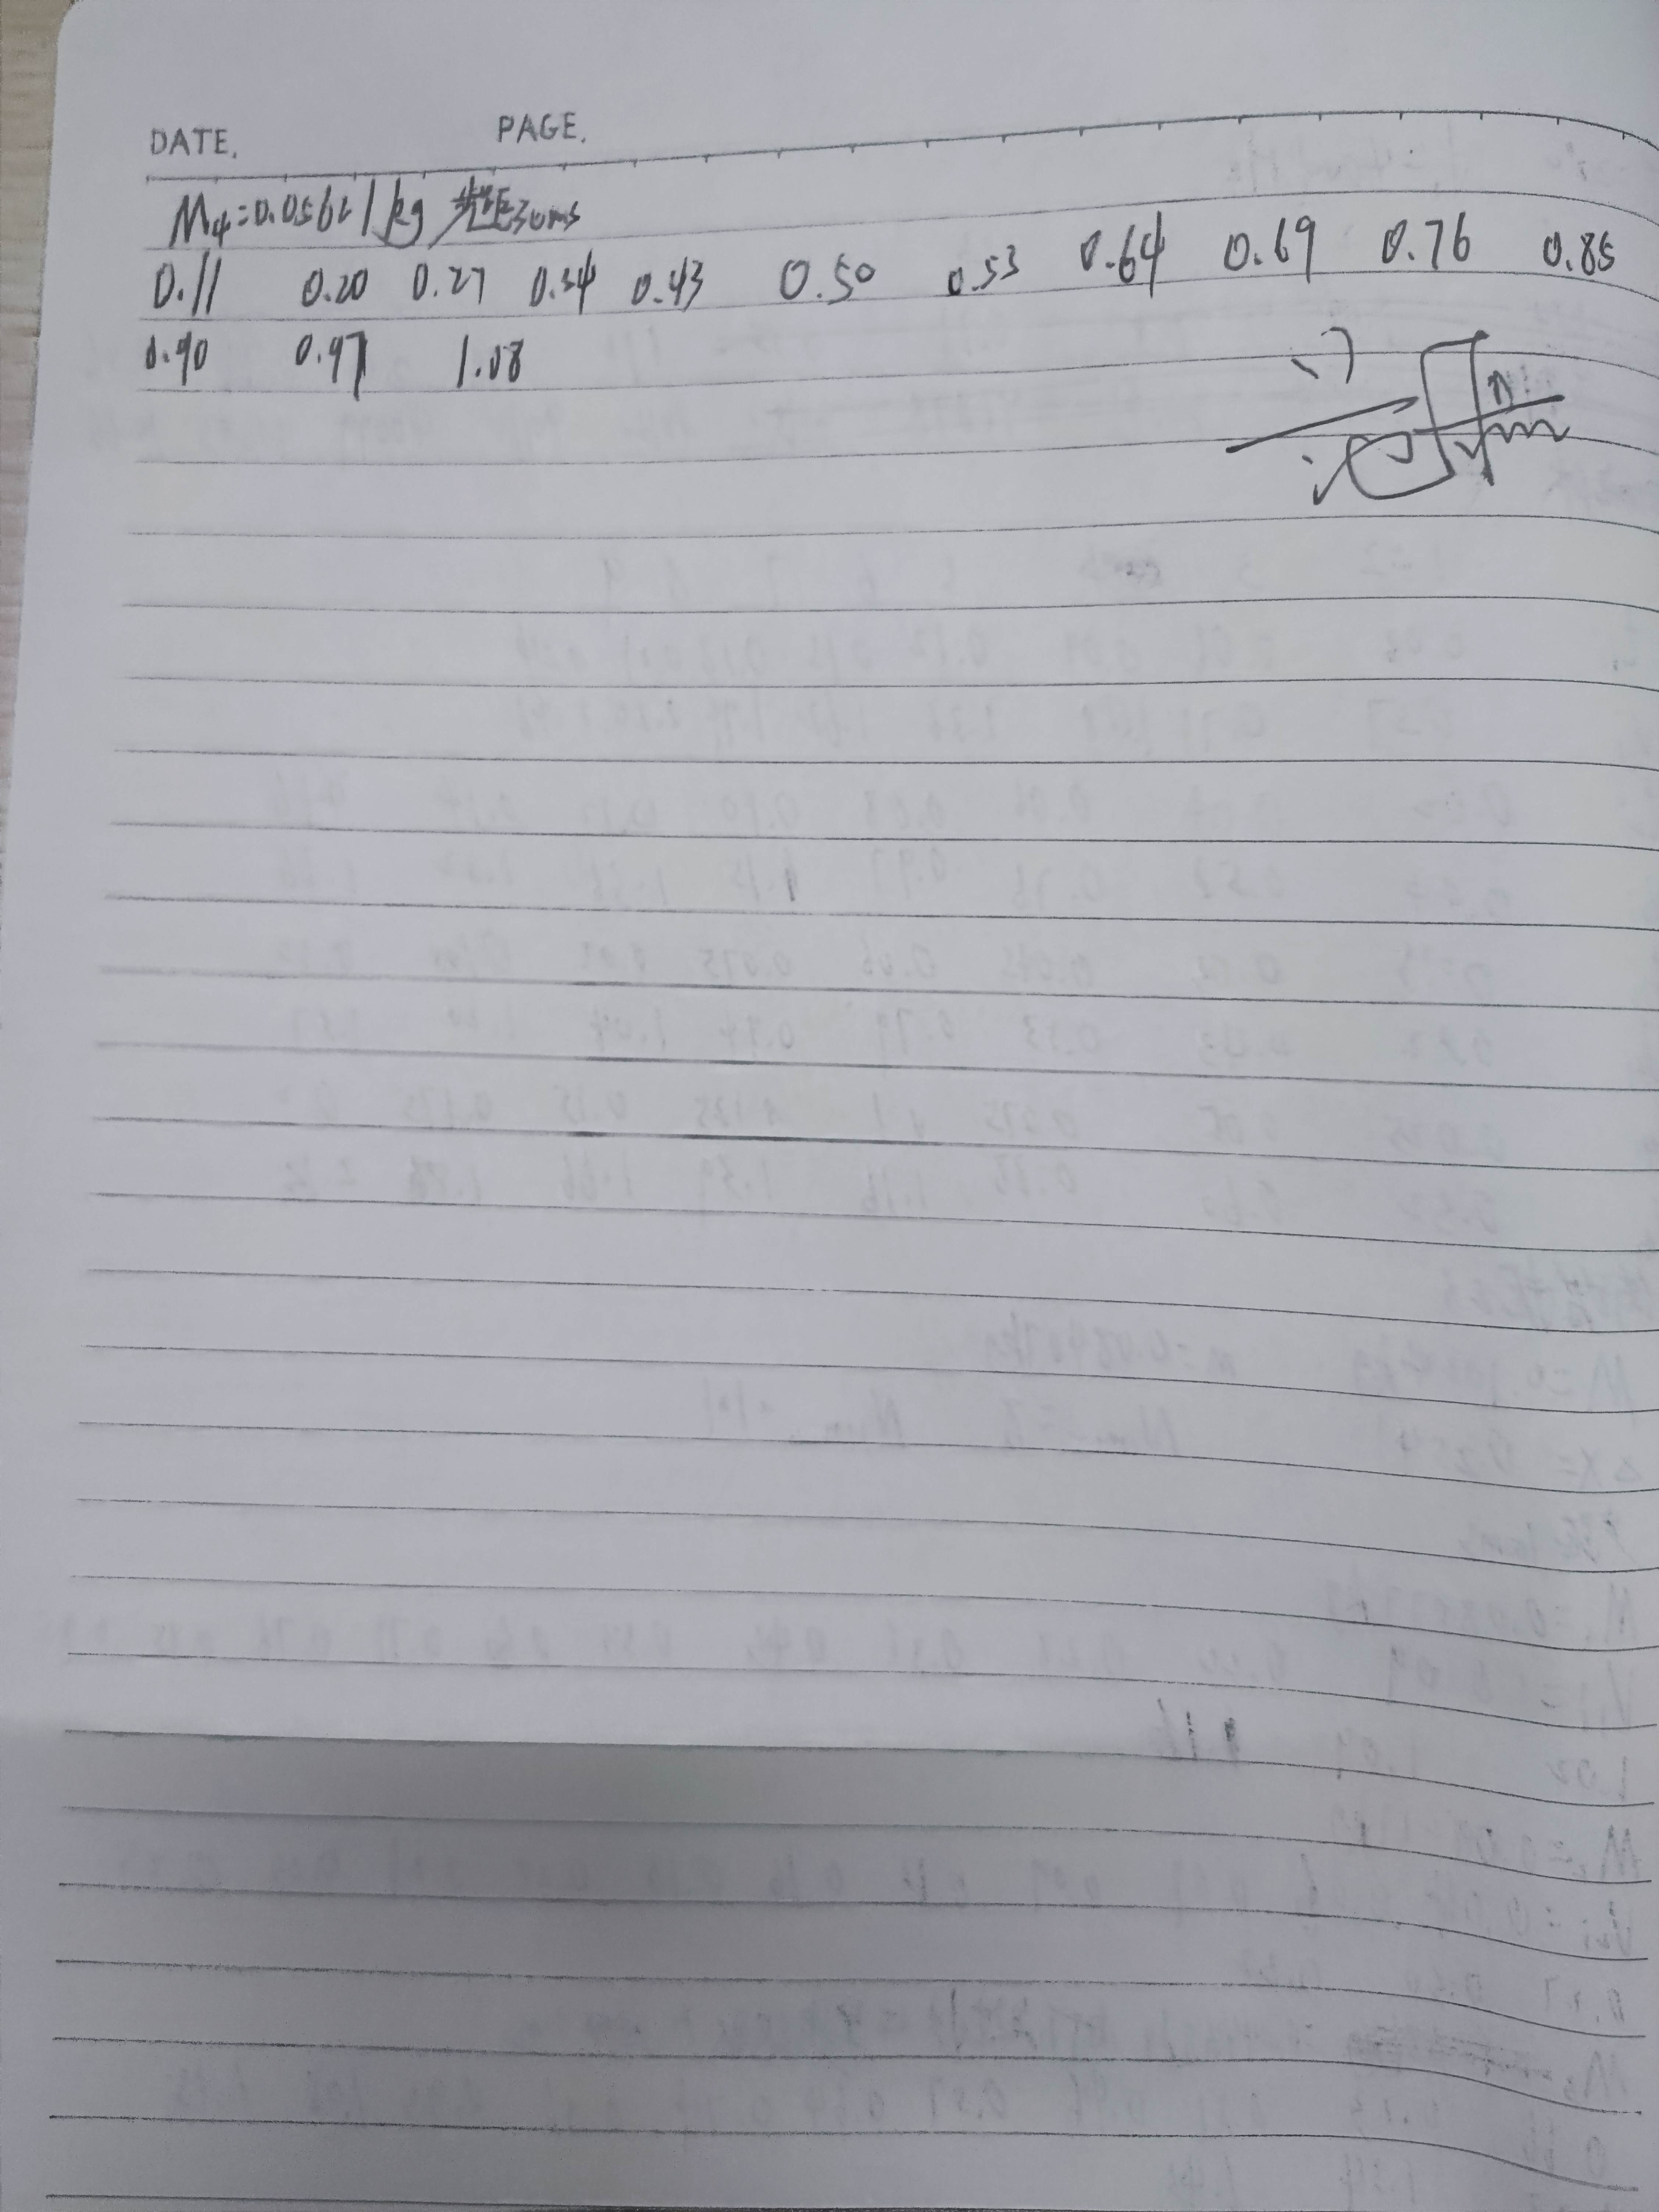
\includegraphics[width=0.4\textwidth]{多普勒原件2.jpg}
%\end{figure}
\subsection*{桌面}
\begin{figure}[H]
	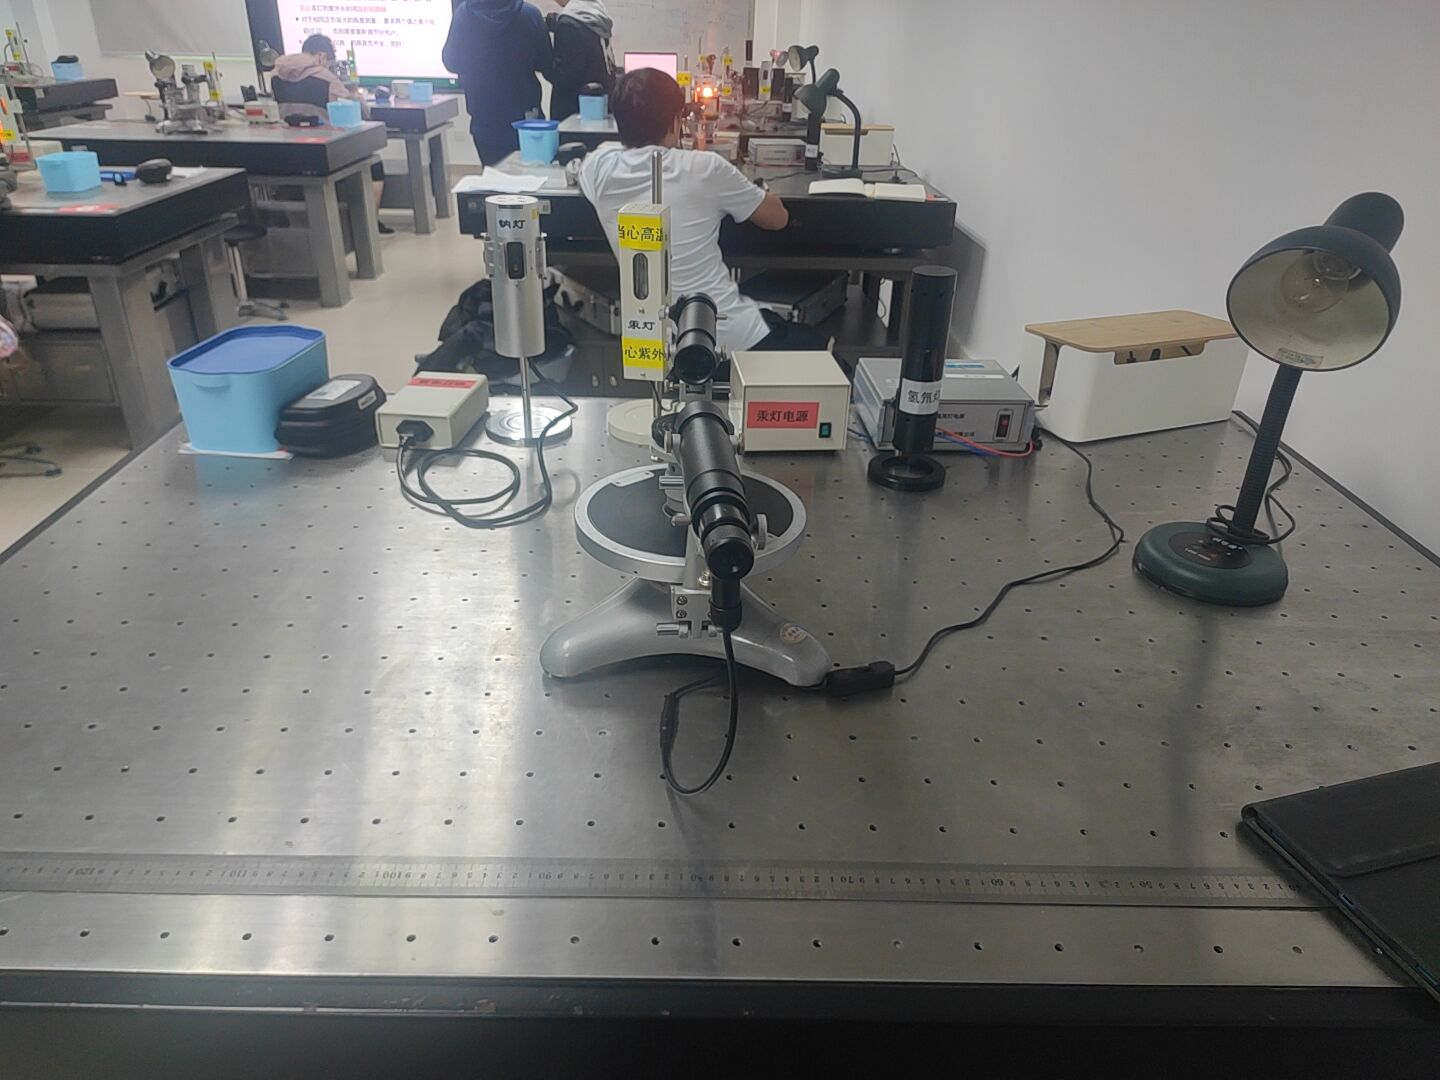
\includegraphics[width=0.95\textwidth]{光栅桌面.jpg}
\end{figure}
\end{document}
